\documentclass[10pt,a4paper]{article}
\usepackage[utf8]{inputenc}
\usepackage[italian]{babel}
\usepackage{amsmath}
\usepackage{amsfonts}
\usepackage{amssymb}
\usepackage{graphicx}
\usepackage[left=2cm,right=2cm,top=2cm,bottom=2cm]{geometry}
\newcommand{\rem}[1]{[\emph{#1}]}

\author{Gruppo AC \\ Federico Belliardo, Giulia Franchi, Francesco Mazzoncini}
\title{Esercitazione N.6: Amplificatore operazionale: circuiti lineari}
\begin{document}
\maketitle
\section{Scopo dell'esperienza}

Misurare le caratteristiche di amplificatori invertenti e non invertenti realizzati con un op-amp TL081 in fig.\ref{pin}.
\begin{figure}[!htb]
  \centering
  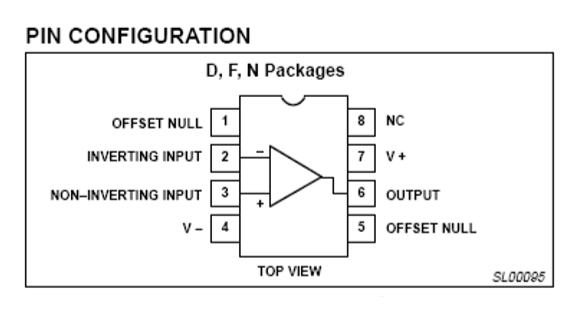
\includegraphics[scale=0.5]{pinrelaz6.png}
\caption{Configurazione pin dell'opAmp.}
\label{pin}
\end{figure}

\section{Amplificatore invertente}
\subsection{Realizzazione circuito}
Si vuole realizzare un amplificatore invertente con un'impedenza di ingresso superiore a $1k\Omega$ e con un amplificazione di 10. 
Per fare ciò abbiamo montato il circuito in fig. \ref{opampinvert}: Tale circuito infatti presenta una  resistenza di ingresso $R_{in}=R_1$ e un'amplificazione  $A_V=-R_2/R_1$ .\\
Si sono scelte $R_1=2.18 \pm 0.02 \, k\Omega$ e $R_2=21.5 \pm0.02 \, k\Omega$ e abbiamo inoltre misurato le  tensioni di alimentazione dell'OpAmp $V_+=14.99 \pm 0.08 \, V$ e $V_-=-15.00 \pm 0.08 \, V$.\\
Con questo circuito la resistenza interna attesa è quindi $R_{in.ATT}= R_1 = 2.18 \pm 0.02 \, k\Omega$ e $A_{V.ATT}= -9.9 \pm 0.1$ in accordo con le richieste.\\

\begin{figure}[!htb]
  \centering
  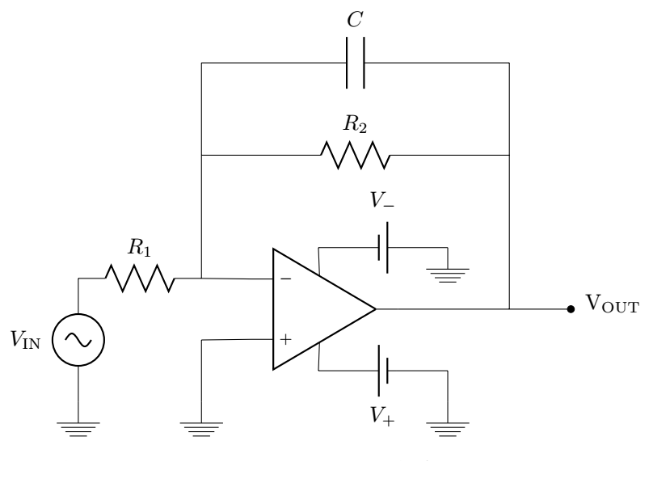
\includegraphics[scale=0.5]{opampinvert.png}
\caption{Schema circuitale amplificatore invertente.}
\label{opampinvert}
\end{figure}

\subsection{Misura del guadagno a frequenza fissata}
Abbiamo misurato per un segnale sinusoidale di frequenza $f=3.00 \pm 0.03 \, kHz$ la tensione picco-picco $V_{OUT}$ in funzione di $V_{IN}$ (sempre picco-picco) riportando i dati nella tabella \ref{tabellaGuadagno}. \\
Abbiamo interrotto la presa dati al valore della tensione in ingresso per il quale abbiamo osservato clipping, misurando però anche il massimo valore della tensione in uscita  $V_{OUT} = 27.0\pm0.2 \, V$, ci saremmo aspettato una tesnsione picco-picco in questo caso limite di $V_{p,p} = 30 \, V$, cioè la differenza delle tensioni di alimentazione.

\begin{table}[!htb]\centering
\begin{tabular}{|c|c|c|c|c|c|}
\hline
$V_{IN} (V)$ & $ \sigma V_{IN} (V)$ & $ V_{OUT} (V)$ & $ \sigma V_{OUT} (V)$ & $A_V$ & $\sigma A_V$\\  
\hline
2.74 & 0.02 & 26.6 & 0.2 & -9.7 & 0.1\\
2.28 & 0.02 & 22.4 & 0.2 & -9.8 & 0.1\\
1.80 & 0.02 & 17.6 & 0.2 & -9.8 & 0.2\\
1.29 & 0.01 & 12.6 & 0.1 & -9.8 & 0.1\\
0.904 & 0.008 & 8.80 & 0.08 & -9.7 & 0.1\\
0.624 & 0.008 & 6.00 & 0.08 & -9.6 & 0.2\\
0.464 & 0.004 & 4.64 & 0.04 & -10.0 & 0.1\\
0.316 & 0.002 & 3.12 & 0.02 & -9.87 & 0.09\\
0.232 & 0.002 & 2.28 & 0.02 & -9.8 & 0.1\\
\hline
\end{tabular}
\caption{Dati delle tensioni $V_{IN}$, $V_{OUT}$ e ampiezze calcolate $A_V$.}
\label{tabellaGuadagno}
\end{table}

Abbiamo eseguito inoltre un grafico di $V_{OUT}$ in funzione di $V_{IN}$ e un fit con una retta riportato in fig. \ref{rettaGuadagno} ricavando come guadagno $A_V=9.74\pm0.04$ \footnote{Nella propagazione degli errori e nel fit si è trascurato l'errore sistematico di calibrazione del  $3\%$ dell'oscilloscopio perchè questo tende a semplificarsi del rapporto di due tensioni.}, compatibile entro l'errore con il guadagno atteso anche se decisamente inferiore.\\

Per il fit si è utilizzata la funzione \emph{curvefit} della libreria \emph{pylab} con l'opzione \emph{$absolute\,sigma = "true"$}, poichè abbiamo considerato gli errori come statistici. Riportiamo di seguito parametri $m$ e $q$ della retta $y=mx+q$, con la relativa matrice di covarianza: $m = 9.74 \pm 0.04$, $q = 0.03\pm 0.03 \, V$,  $ \Sigma_{ij} = \left( \begin{array}{cc}
2.10 \cdot 10^{-3} & -7.54 \cdot 10^{-4} \\ 
-7.54 \cdot 10^{-4} & 4.37 \cdot 10^{-4}\\
\end{array} \right)$. Con un $\chi^2/ndof = 8.4/7$.\\


\begin{figure}[!htb]
  \centering
  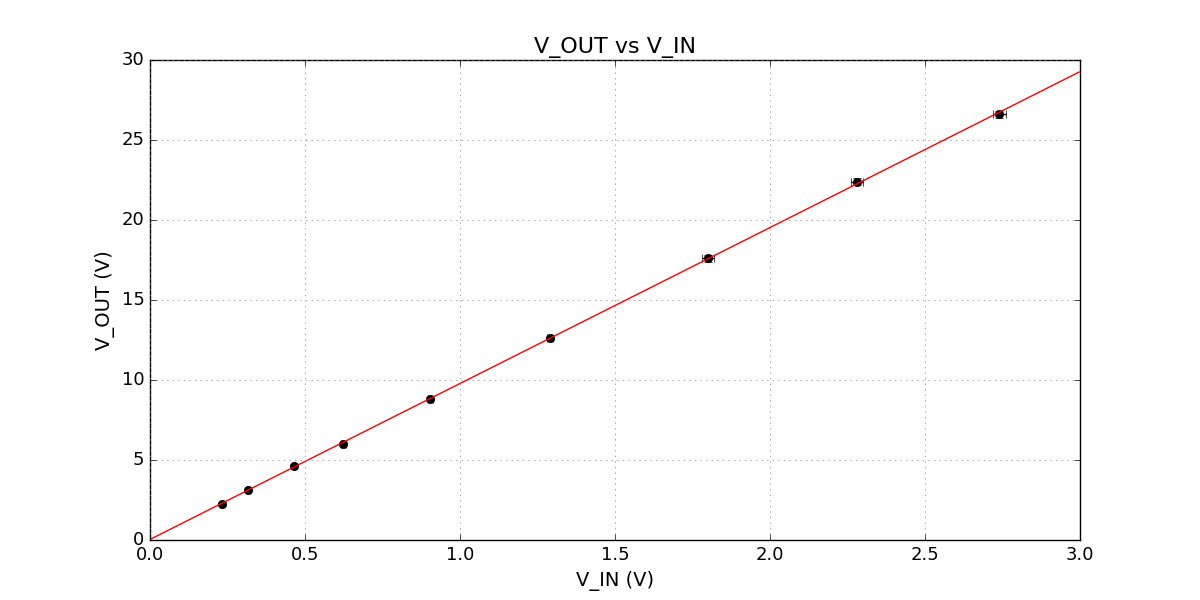
\includegraphics[scale=0.6]{plotGuadagno.png}
\caption{Fit della tensione $V_{OUT}$ in funzione di $V_{IN}$.}
\label{rettaGuadagno}
\end{figure}

\subsection{Misura dell'impedenza d'ingresso}
Ci aspettiamo una resistenza di ingresso pari a $R_1$.
Abbiamo misurato la tensione di uscita del circuito a $V_{IN}=1.00 \pm 0.01 \, V$, in modo da evitare fenomeni di clipping, dapprima con lo stesso circuito, poi successivamente aggiugendo una resistenza $R_S=2.19 \pm 0.02 \, k \Omega$ \footnote{$R_S$ è stata scelta dello stesso ordine della resistenza interna attesa, in modo da non alterare troppo il circuito, ma più grande, in modo da minimizzare l'incertezza} in serie al generatore di funzioni, ottenendo rispettivamente $V_1=9.68 \pm 0.08 \, V$ e $V_2= 4.88 \pm 0.04 \, V$ Dalla formula del partitore otteniamo $R_S/R_{IN}=\frac{V_1}{V_2}-1$, cioè:
$R_{IN} = R_S \frac{1}{\frac{V_1}{V_2}-1} = 2.22 \pm 0.06 \, k \Omega$, in buon accordo con quella prevista entro l'errore sperimentale.

\section{Risposta in frequenza del circuito e slew rate}
\subsection{Misura della risposta in frequenza}

Abbiamo studiato la risposta in frequenza del circuito misurando $V_{OUT}$ al variare della frequenza (scegliere l'intervallo) con $V_{IN}=0.800 \pm 0.008 \, V$  sinusoidale fissata. \footnote{$V_{IN}$ è stata scelta in modo da non avere effetti di distorsione e ci siamo accertati che l'ampiezza del segnale in ingresso rimanesse costante al variare della frequenza, avendo cura in caso di necessità di agire sul generatore di funzioni in modo da avere il segnale voluto.} \\
I dati ottenuto sono stati riportati nella tabella \ref{tabellaBode} e sono stati graficati in un diagramma di Bode in fig. \ref{graficoBode}.\\
Le frequenze sono state misurate con il frequenzimetro dell'oscilloscopio, ad esse si è assegnato un errore dell'$1\%$, poiché è anche l'errore con cui riusciremmo a stimare il periodo con il cursore dei tempi.\\

\begin{table}[!htb]\centering
\begin{tabular}{|c|c|c|c|}
\hline
$f (kHz)$ & $\sigma f (kHz) $ & $ V_{OUT} (V)$ & $\sigma V_{OUT} (V)$\\
\hline
0.00511 & 0.00005 & 7.84 & 0.08\\
0.0098 & 0.0001 & 7.76 & 0.08\\
0.0292 & 0.0003 & 7.76 & 0.08\\
0.102 & 0.001 & 7.92 & 0.08\\
0.307 & 0.003 & 7.92 & 0.08\\
1.02 & 0.01 & 8.00 & 0.08\\
3.04 & 0.03 & 8.00 & 0.08\\
10.2 & 0.1 & 8.00 & 0.08\\
30.9 & 0.3 & 7.84 & 0.08\\
48.2 & 0.5 & 7.52 & 0.04\\
92.7 & 0.9 & 7.04 & 0.04\\
156 & 2 & 6.36 & 0.04\\
212 & 2 & 5.64 & 0.04\\
312 & 3 & 4.36 & 0.02\\
505 & 5 & 2.98 & 0.02\\
704 & 7 & 2.16 & 0.02\\
1000 & 10 & 1.560 & 0.008\\
1600 & 20 & 0.904 & 0.008\\
\hline
\end{tabular}
\caption{Frequenze $f$ del segnale il ingresso e relativo $V_{OUT}$ picco-picco misurato.}
\label{tabellaBode}
\end{table}

Abbiamo notato che il circuito si comporta come un filtro passa-basso ed abbiamo quindi  eseguito un fit con la funzione $ A=\frac{A_{MAX}}{\sqrt{1+(f/f_t)^2}}$.

\begin{figure}[!htb]
  \centering
  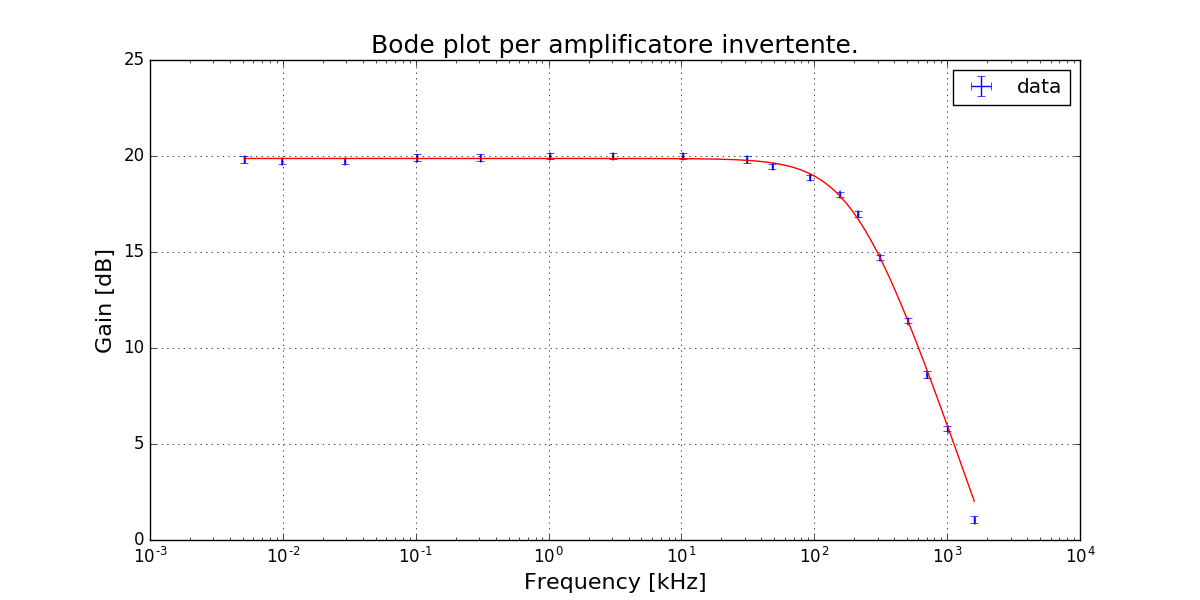
\includegraphics[scale=0.6]{bodePlot.png}
\caption{Plot di Bode amplificatore invertente.}
\label{graficoBode}
\end{figure}

Il fit fornisce: $f_T = 206 \pm 4 \, kHz$ e $A_{max} = 9.85 \pm 0.04$, con matrice di covarianza:\\
$ \Sigma_{ij} = \left( \begin{array}{cc}
14.1 & -6.23 \cdot 10^{-2} \\ 
-6.23 \cdot 10^{-2} & 1.57 \cdot 10^{-3}\\
\end{array} \right)$. Con un $\chi^2/ndof = 4.46/16$.\\

Il guadagno massimo anche in questo fit è compatibile con quello atteso, $A_{V.ATT}= -9.9 \pm 0.1$.

\subsection{Slew rate}
Abbiamo impostato il generatore di funzioni in modo che fornisse al circuito un’onda quadra. Si è studiato l'andamento di $V_{OUT}$ nella parte del segnale corrispondente al transiente fra i due stati dell’onda: la tensione osservata presenta inizialmente un andamento qualitativamente esponenziale, successivamente un andamento lineare per poi rallentare in prossimità del suo valore limite.\\
Nella zona di crescita lineare si è dunque presa una misura della differenza di tensione $dV_{OUT} = 1.00 \pm 0.04 \, V$ relativa a un piccolo intervallo di tempo $dt=90 \pm 1 \, ns$. Dal loro rapporto si ottiene il valore dello $\emph{slew rate}= 11.1 \pm 0.5 \, \frac{V}{\mu s}$ \footnote{Per calcolare lo \emph{slew rate}, nell'errore sulle misure di tensione è stato considerato anche l'errore sistematico del $3\%$ dell'oscilloscopio.}. Il \emph{datasheet} dell'integrato riporta un valore nominale di $13 \frac{V}{\mu s}$ che non è compatibile entro l'errore con il valore misurato, ma un valore di $11 \frac{V}{\mu s}$ rientra nella variabilità del processo di costruzione.

\section{Amplificatore non invertente}
Abbiamo montato il circuito in fig. \ref{opampnoninvert} con $R_1=218 \pm 2 \,  \Omega$ e  un potenziometro di resistenza massima $P_{1_{MAX}}= 97.8 \pm 0.8 \, k\Omega$. La tensione di ingresso è stata fissata a $V_{IN} = 340 \pm 2 \, mV$.
Il valore di $V_{OUT}$ nella tabella si riferisce al massimo guadagno ($A_{max}$) ottenibile, mentre la frequenza di taglio $f_H$ è stata determinata cercando a quale frequenza il  guadagno è $A\,(dB)= A_{max}\,(dB) - 3 \,dB$. Questo  è in linea con l'ipotesi che la funzione di traferiemento dell'amplificatore  sia della stessa forma di un sitema passa-basso. Si vuole verificare l'ipotesi che il prodotto-banda guadagno definito come $BG = A_{max} f_H$ rimanga costante al variare della frequenza. 

\begin{figure}[!htb]
  \centering
  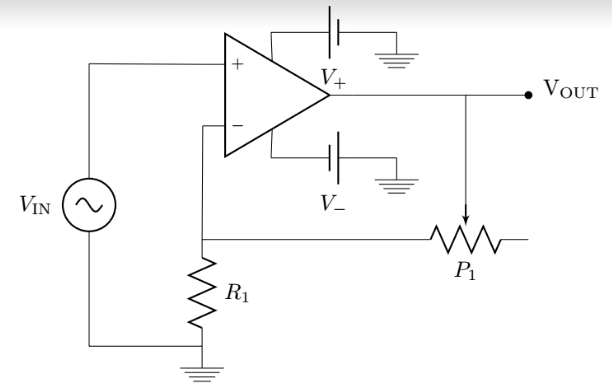
\includegraphics[scale=0.5]{opampnoninvert.png}
\caption{Schema operatore amplificazionale non invertente.}
\label{opampnoninvert}
\end{figure}

\begin{table}[!htb]\centering
\begin{tabular}{|c|c|c|c|c|c|c|c|}
\hline
$V_{OUT} (V)$ & $\sigma V_{OUT} (V)$ & $ f_H(kHz) $ & $ \sigma f_H(kHZ)$ & $A_{max}$ & $\sigma A_{max}$ & $BG (MHz)$ & $\sigma BG (MHz)$\\    
\hline
17.4 & 0.2 & 41.0 & 0.4 & 51.2 & 0.7 & 2.10 & 0.03\\
6.56 & 0.02 & 111 & 1 & 19.3 & 0.1 & 2.14 & 0.01\\
1.96 & 0.02 & 380 & 4 & 5.76 & 0.07 & 2.19 & 0.03\\
4.00 & 0.04 & 187 & 2 & 11.8 & 0.1 & 2.20 & 0.03\\
13.0 & 0.1 & 55.0 & 0.6 & 38.2 & 0.4 & 2.10 & 0.02\\
\hline
\end{tabular}
\caption{Tensioni massime in uscita, frequenze di taglio e prodotto banda-guadagno.}
\label{tabellaBG}
\end{table}

Come si può vedere dalla tabella il valore del prodotto BG rimane circa costante, è stato sottostimato l'errore sulla nostra capacità di individuazione della frequenza di taglio avendo inserito solamente l'errore di misura dell'$1\%$, e non un errore dovuto al fatto che la frequenza selezionata per il dato guadagno calcolato non fosse precisa.
Il valore medio del prodotto banda-guadagno è: $BG = 2.15\pm0.02 \, MHz$.

\section{Circuito integratore}
Abbiamo utilizzato come segnale di ingresso fornito dal generatore di funzioni  un onda sinusoidale di ampiezza $V_{IN}=460 \pm 4 \, mV$ \footnote{Anche in questo caso abbiamo eseguito le accortezze sperimentali descritte nella nota precedente sul controllo della tensione in ingresso $V_{IN}$.}. I componenti scelti per realizzare l'integratore sono: $R_1 = 984 \pm 8 \Omega$, $R_2 = 11.8 \pm 0.1 k\Omega$ e $C = 45 \pm 2$.\\

\begin{figure}[!htb]
  \centering
  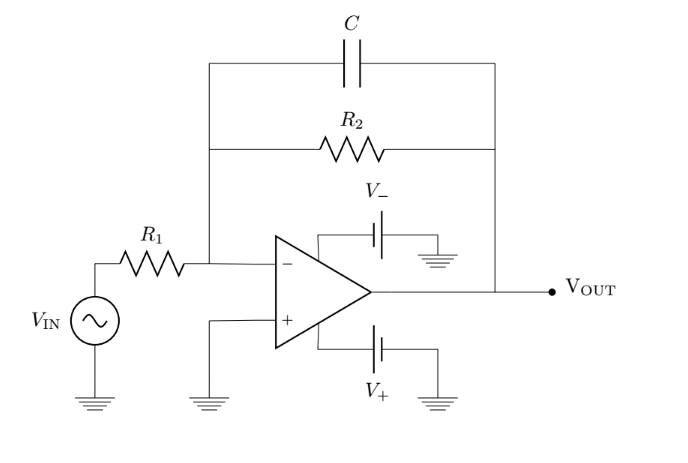
\includegraphics[scale=0.25]{integratore.png}
\caption{Schema di circuito integratore con opAmp}
\end{figure}


Si sono misurate la tensione in uscita e lo sfasamento al variare della frequenza, i dati sono riportati nella tabella \ref{tabellaIntegratore}.\\

\begin{table}[!htb]\centering
\begin{tabular}{|c|c|c|c|c|c|}
\hline$f \, (Hz)$ & $ \sigma f \, (Hz)$ & $V_{OUT} \, (V)$ & $\sigma V_{OUT} \, (V)$ & $\phi (\pi \, rad)$ & $\sigma \phi (\pi \,  rad)$\\
\hline
2.12 & 0.02 & 5.44 & 0.04 & 0.98 & 0.02\\
5.23 & 0.05 & 5.44 & 0.04 & 1.00 & 0.02\\
19.1 & 0.2 & 5.44 & 0.04 & 0.98 & 0.02\\
59.2 & 0.6 & 5.40 & 0.04 & 0.93 & 0.03\\
196 & 2 & 4.60 & 0.04 & 0.81 & 0.01\\
497 & 5 & 2.84 & 0.02 & 0.69 & 0.02\\
337 & 3 & 3.64 & 0.02 & 0.75 & 0.02\\
907 & 9 & 1.74 & 0.02 & 0.60 & 0.02\\
1990 & 20 & 0.808 & 0.008 & 0.56 & 0.02\\
\hline
\end{tabular}
\caption{Dati di tensione $V_{OUT}$ e sfasamento per l'integratore.}
\label{tabellaIntegratore}
\end{table}


\begin{figure}[!htb]
\centering
  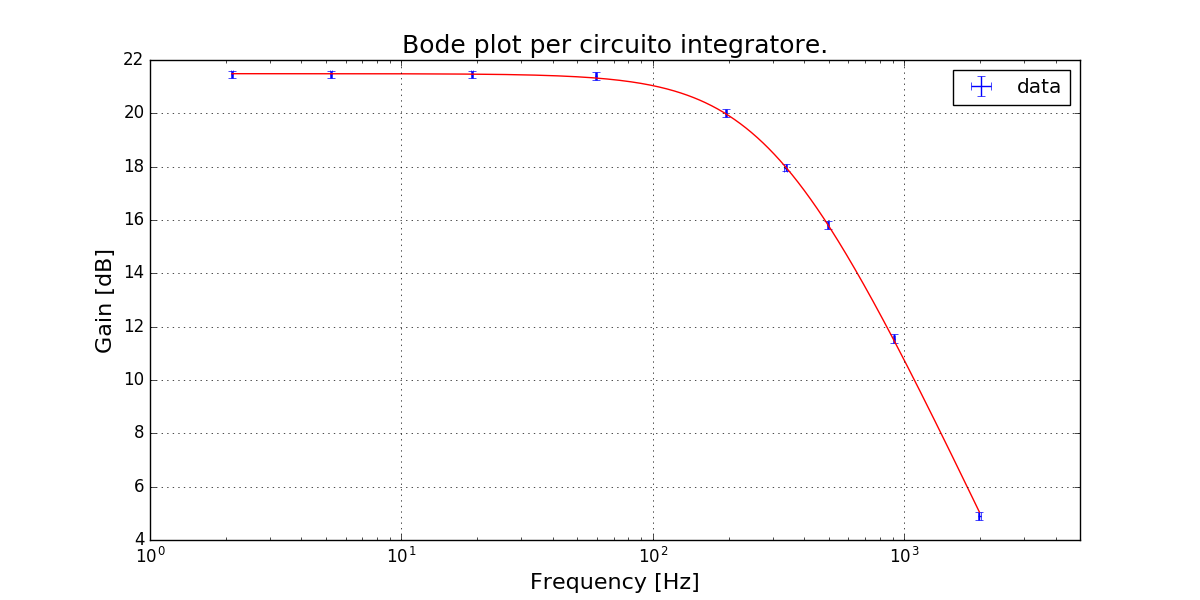
\includegraphics[scale=0.6]{bodeIntegratore.png}
\caption{Plot di Bode per il circuito integratore.}
\label{plotIntegratore}
\end{figure}

\begin{figure}[!htb]
\centering
  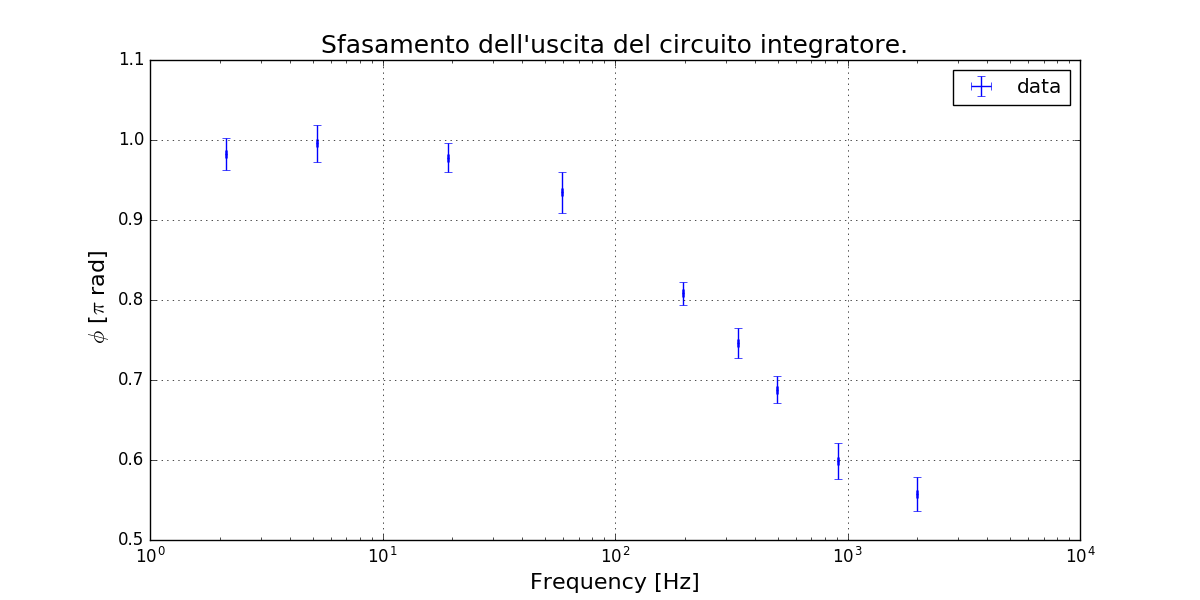
\includegraphics[scale=0.6]{integratoreSfasamento.png}
\caption{Sfasamento della risposta per il circuito integratore.}
\label{plotIntegratore2}
\end{figure}


Il fit riportato nel grafico \ref{plotIntegratore} è stato eseguito con la funzione di trasferimento del passa-basso: $ A=\frac{A_{max}}{\sqrt{1+(f/f_t)^2}}$, otteniamo i valori: $f_t = 303 \pm 2 \, Hz$ e $A_{max} = 11.87 \pm 0.02$, la matrice di covarianza è:\\ $ \Sigma_{ij} = \left( \begin{array}{cc}
4.27 & -2.45 \cdot 10^{-2} \\ 
-2.45 \cdot 10^{-2} & 5.31 \cdot 10^{-4}\\
\end{array} \right)$. Con un $\chi^2/ndof = 1.36/7$.\\
Il $\chi^2$ è inferiore al valore atteso questo significa che gli errori sono stati sovrastimati. 

Il valore del guadagno massimo è decisamente superiore a quello atteso dal rapporto tra le resistenze: $A_{V.ATT}= -9.9 \pm 0.1$ , questo perchè la legge \emph{fittata} per l'integratore è da considerarsi un'approssimazione.

Sia il plot di bode che lo sfasamento sono in linea con quanto atteso per un circuito passa-basso. Lo sfasamento è dato da $\phi = \pi - arctan \left( \frac{f}{f_0} \right)$, dove si aggiunge il $\pi$ perchè vi è inversione del segnale.


\paragraph{Risposta all'onda quadra.} Si è studiata la risposta del circuito ad un'onda quadra di frequenza $f = 10 \, kHz$ come si vede nella fig. \ref{integratore10}, le tensioni picco-picco in ingresso e uscita sono rispettivamente: $V_{IN} = 476 \pm 4 \, mV$ e $V_{OUT} = 256 \pm 2 \, mV$, dunque il guadagno a questa frequenza è $A_{10\, kHz} = 0.538 \pm 0.006$. Per un'ond sinusoidale a questa frequenza ci aspetteremmo $A_{fit} = 0.35 \pm 0.02$, ma chiaramente l'onda quadra contiene tutte le armonihe dispari nello sviluppo di Fourier, per ognuna delle quali bisogna calcolare il guadagno, quindi non ci aspettiamo che i due risultati siano simili.

\begin{figure}[!htb]
\centering
  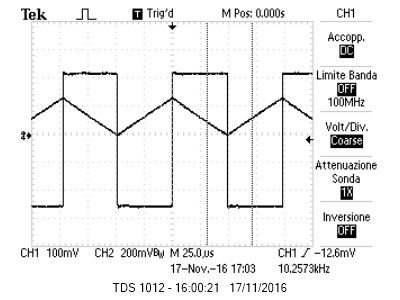
\includegraphics[scale=1.0]{immagini/integratore.png}
\caption{Risposta dell'integratore a un'onda quadra a $10\,kHz$}
\label{integratore10}
\end{figure}

Per una frequenza di circa $f = 200 \, kHz$, si osserva che la risposta dell'integratore a un'onda quadra è un segnale a pinna di squalo (cioè presenta la caratteristica salita esponenziale della carica e scarica di un condensatore), come si vede nella fig. \ref{squalo}. Questo è dovuto al fatto che la frequenza fondamentale (essendo al di sotto della frequenza di taglio) viene amplificata all'uscita, mentre le arminiche superiori vengono integrate dando il tipico comportamento esponenziale.

\begin{figure}[!htb]
\centering
  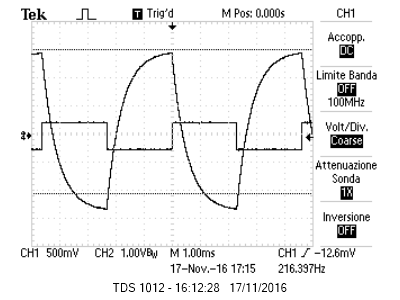
\includegraphics[scale=1.0]{immagini/pinnasqualo.png}
\caption{Risposta a pinna di squalo dell'integratore.}
\label{squalo}
\end{figure}

A frequenze ancora più basse (dell'ordine di $f = 10 \,Hz$) il circuito si comporta come un amplificatore invertente come ci si aspetta dal segno meno nella formula dell'amplificazione, si può vedre la fig. \ref{bassafreq}.
\begin{figure}[!htb]
\centering
  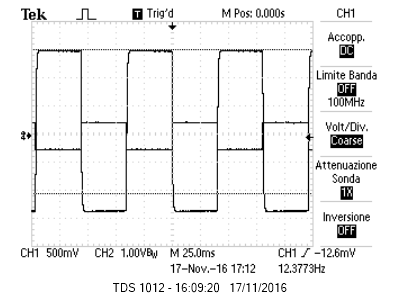
\includegraphics[scale=1.0]{immagini/bassafreqondaquadra.png}
\caption{Risposta a bassissima frequenza del circuito integratore.}
\label{bassafreq}
\end{figure}

Senza la resistenza $R_2$ la funione di trasferimento del circuito sarebbe: $A = -\frac{1}{\omega RC}$, $R_2$ serve proprio per spostare il polo dallo zero della frequenza (stabilizzando il circuito) e introdurre quindi un guadagno massimo a frequenza nulla. La resistenza $R_2$ è quindi responsabile della presenza di una frequenza di taglio per l'integratore.

\section{Circuito derivatore}
\paragraph{Bode plot.} Si è realizzato il circuito derivatore come in fig. \ref{derivatore}, sposatndo il condensatore in serie alla resistenza $R_1$. Si sono presi dati a varie requenze riportati nella tabella \ref{derivatore}, lavorando con una tensione di ingresso $V_{IN} = 448 \pm 4 \, mV$.\\

\begin{figure}[!htb]
\centering
  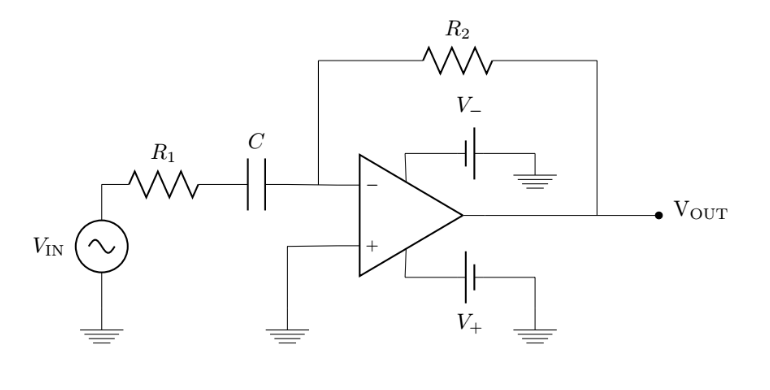
\includegraphics[scale=0.25]{derivatore.png}
\caption{Circuito derivatore con OpAmp}
\label{derivatore}
\end{figure}

\begin{table}[!htb]\centering
\begin{tabular}{|c|c|c|c|c|c|}
\hline$f \, (Hz)$ & $ \sigma f \, (Hz)$ & $V_{OUT} \, (V)$ & $\sigma V_{OUT} \, (V)$ & $\phi (\pi \, rad)$ & $\sigma \phi (\pi \, rad)$\\
\hline
695 & 7 & 1.25 & 0.01 & 0.46 & 0.01\\
296 & 3 & 2.56 & 0.02 & 0.60 & 0.02\\
49.5 & 0.5 & 5.12 & 0.04 & 0.921 & 0.004\\
19.7 & 0.2 & 5.16 & 0.04 & 0.976 & 0.008\\
9.8 & 0.1 & 5.00 & 0.04 & 0.913 & 0.008\\
68.9 & 0.7 & 5.00 & 0.04 & 0.879 & 0.006\\
28.5 & 0.3 & 5.24 & 0.04 & 0.975 & 0.002\\
5.01 & 0.05 & 4.40 & 0.04 & 0.800 & 0.004\\
0.912 & 0.009 & 1.30 & 0.01 & 0.577 & 0.008\\
1.88 & 0.02 & 2.42 & 0.04 & 0.65 & 0.02\\
0.393 & 0.004 & 0.576 & 0.008 & 0.53 & 0.02\\
0.0920 & 0.0009 & 0.134 & 0.001 & 0.52 & 0.02\\
\hline
\end{tabular}
\caption{Dati di tensione $V_{OUT}$ e sfasamento per il derivatore.}
\label{derivatore}
\end{table}

\begin{figure}[!htb]
\centering
  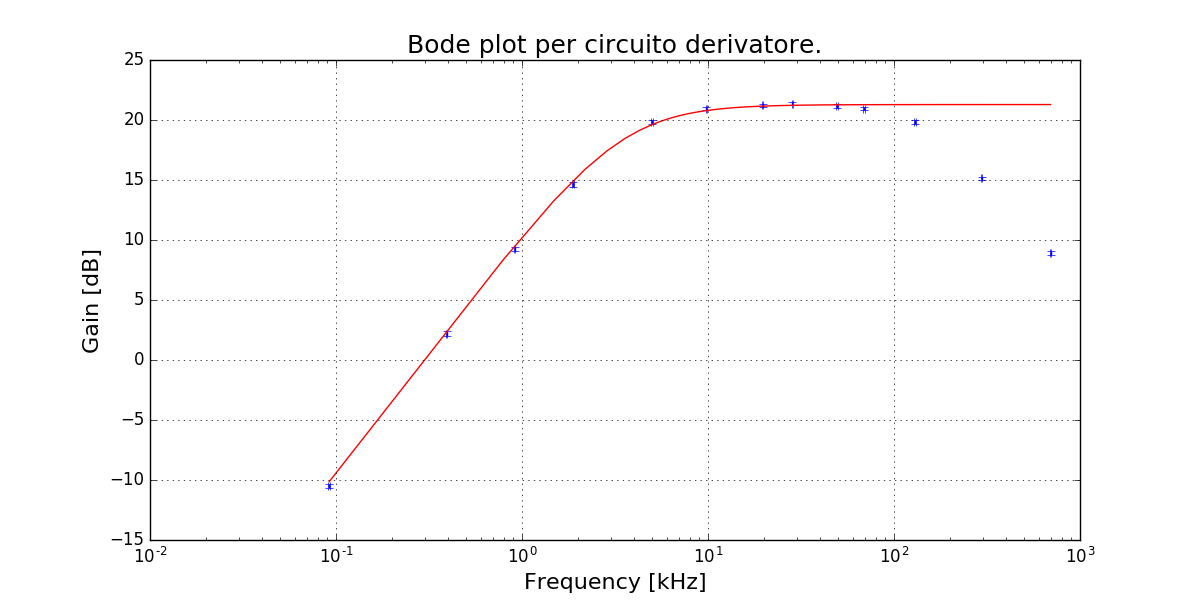
\includegraphics[scale=.6]{bodeDerivatore.png}
\caption{Bode plot per il circuito derivatore.}
\label{bodeDerivatore}
\end{figure}

\begin{figure}[!htb]
\centering
   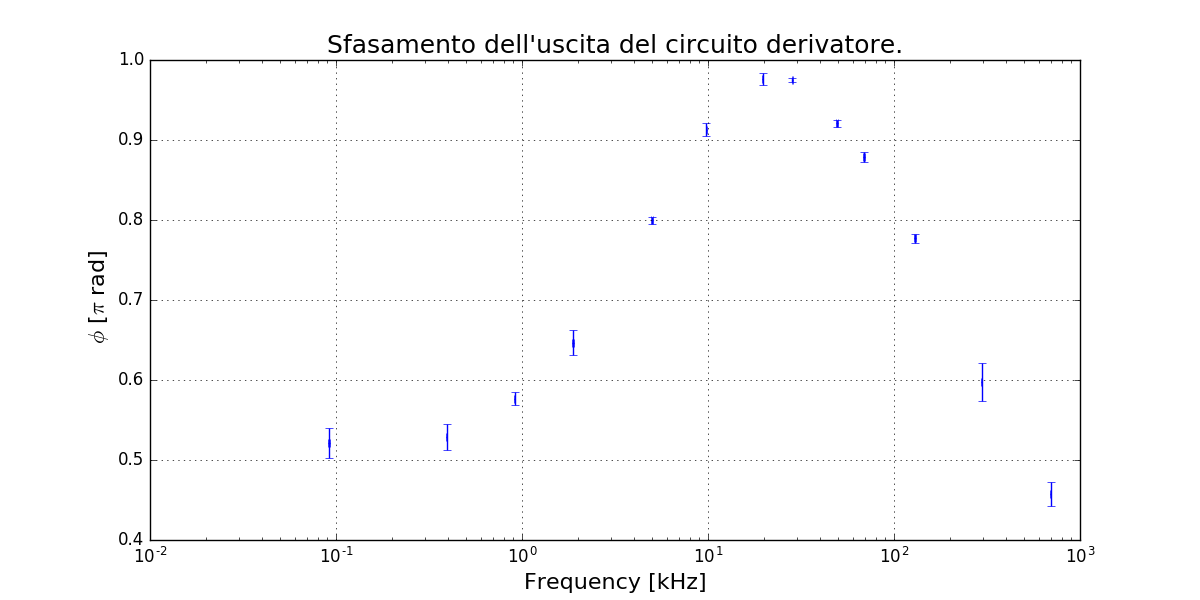
\includegraphics[scale=.6]{derivatoreSfasamento.png}
\caption{Sfasamento per il circuito derivatore.}
\label{sfasamentoDerivatore}
\end{figure}

Si è eseguito un fit della funzione di trasferimento nota per il circuito passa-alto, cioè:
$ A=\frac{A_{max}}{\sqrt{1+(f_t/f)^2}}$, l'algoritmo ha fornito i valori ottimali: $f_t = 3.4 \pm 0.1 \, kHz$ e $A_{max} = 11.6 \pm 0.1$, la matrice di covarianza è: $ \Sigma_{ij} = \left( \begin{array}{cc}
 0.018 & -6.75 \cdot 10^{-3} \\ 
-6.75 \cdot 10^{-3} & 0.011\\
\end{array} \right)$. 
Con un $\chi^2/ndof = 22/8$.\\
Il $\chi^2$ ottenuto è maggiore del valore atteso, poichè ad alte frequenze (sopra la frequenza di taglio) osserviamo che il comportamento dell'opAmp si discosta dal comportamento ideale di sistema passa-alto, come si può vedere dagli ultimi dati presi sul grafico dello sfasamento.

Il valore del guadagno massimo è decisamente superiore a quello atteso dal rapporto tra le resistenze: $A_{V.ATT}= -9.9 \pm 0.1$ , questo perchè la legge \emph{fittata} per il derivatore è da considerarsi un'approssimazione.

Sia il plot di bode che lo sfasamento sono in linea con quanto atteso per un circuito passa-alto per basse frequenze. Lo sfasamento è dato da $\phi = arctan \left( \frac{f_0}{f} \right) - \pi$, dove si aggiunge il $\pi$ perchè vi è inversione del segnale. Alle alte frequenze (ordine delle centinaia di $kHz$) il comportamento del circuito devia da quello ideale. Sappiamo che per alte frequenze l'amplificazione di ogni sistema fisico deve andare a 0, dunque il guadagno a $-\inf$ come si vede succede nel Bode. Anche lo sfasamento devia considerevolmente dal valore di $\pi$ atteso ad alta frequenza.

\paragraph{Risposta all'onda triangolare.} Come si vede nella fig. \ref{derivatore} per frequenze di $f = 100\,Hz$ il sistema si comporta bene come un derivatore. L'onda quadra presenta come una modulazione esponenziale dovuta probabilmente alla scarica del condensatore.

\begin{figure}[!htb]
\centering
   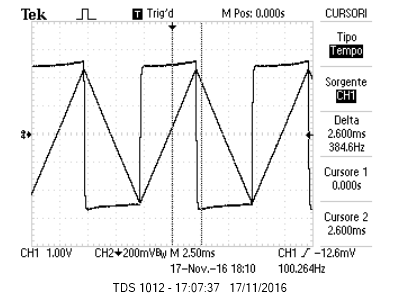
\includegraphics[scale=1.0]{immagini/derivatore.png}
\caption{Risposta del derivatore ad un'onda tringolare di $100\,Hz$.}
\label{derivatore100}
\end{figure}

A questa frequenza abbiamo preso una misura della tensione in ingresso e uscita ottenendo: $V_{IN} = 4.68 \pm 0.02 \, V$, $V_{OUT} = 1.02 \pm 0.02 \, V$, che danno un valore per l'amplificazione: $A = 0.218 \pm 0.004$, da confrontare con il valore atteso per un segnale sinusodale: $A = 0.34 \pm 0.05$. I due valori non sono in accordo perchè chiaramete l'onda quadra non è un armonica pura, bisognarebbe coniderare l'amplificazione per ogni componente.

Alle basse frequenze (circa $f = 20 \, Hz$) il circuito si comporta come un ottimo derivatore, come si vede nella fig. \ref{ottimoDerivatore}

\begin{figure}[!htb]
\centering
   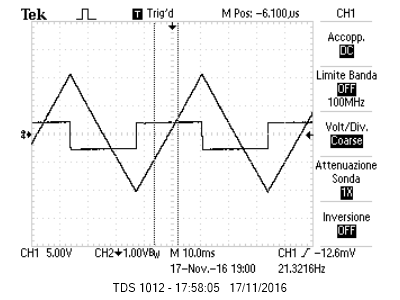
\includegraphics[scale=1.0]{immagini/bassafreqderivatore.png}
\caption{Risposta del derivatore ad un'onda tringolare di $20\,Hz$.}
\label{ottimoDerivatore}
\end{figure}

Abbiamo osservato che per frequenze di circa $500 \, Hz$ il comportamento del circuito non è più quello ideale di un derivatore (per un'onda triangolare) perchè l'onda è costituita dalle armoniche dispari, quindi le componenti ad alta frequenza sono amplificate senza essere derivate, come si può vedere in fig. \ref{derivatore500} (il segnale sembra a pinna di squalo). A riprova di ciò per un segnale sinusoidale di $500 \,Hz$ il comportamento è visibilmente lineare ed è quello di un derivatore. 

\begin{figure}[!htb]
\centering
   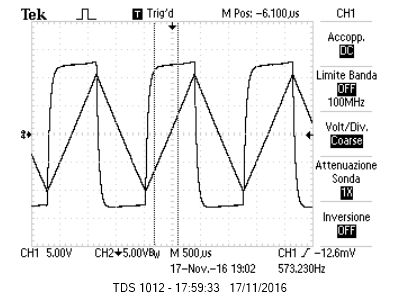
\includegraphics[scale=1.0]{immagini/freq500derivatore.png}
\caption{Risposta del derivatore ad un'onda tringolare di $500\,Hz$.}
\label{derivatore500}
\end{figure}

A riprova di questa interpretazione per altissime frequenze (intorno a $f=3.3\,kHz$) l'uscita del segnale presenta evidentemente la caratteristica forma a pinna di squalo, dunque le alte frequenze sono state amplificate.

E' stato stimato lo \emph{slew-rate} per la risposta ad un'onda triangolare di frequenza $f=277 \, kHz$. L'uscita è un'onda triangolare limitata in frequenza dallo \emph{slew rate} dell'opAmp, le misure con i cursori hanno dato: $dV = 1.00 \pm 0.03 \, V$ e $dt = 88 \pm 4 \, ns$, da queste stimiamo $ \emph{slew rate} = 11.4 \pm 0.6 \, \frac{V}{\mu s}$, che è compatibile con il valore precedentemente misurato.  

Senza la resistenza $R_1$ la funione di trasferimento del circuito sarebbe: $A = - \omega RC$, $R_1$ serve proprio per spostare il polo dallo zero della frequenza (stabilizzando il circuito) e introdurre quindi un guadagno massimo a frequenza "infinita". La resistenza $R_1$ è quindi responsabile della presenza di una frequenza di taglio per il derivatore.

\end{document}